\subsection{sCenario and gOal based SysteM develOpment methoD (COSMOD) (FDD)}\label{scgo}
COSMOD-Requirements Engineering (COSMOD-RE) beschreibt ein iteratives Vorgehen zum gleichzeitigen Design von Anforderungen und Software-Architektur. Kerngedanke bei COSMOD-RE ist eine Aufteilung in vier Hierarchiestufen, wo sowohl Architektur als auch Anforderungen definiert werden. In diesen vier Hierarchiestufen wird einerseits aus der Anforderungssicht und andererseits aus der Architektursicht betrachtet, welche Anforderungen und Komponenten dem System zuzuordnen sind.\\

\subsubsection{Ziele der Methode}
Kernziel von COSMOD-RE ist es die Entwicklung von Anforderungs- und Architekturartefakten für softwareintensive eingebettete Systeme zu unterstützen. Ein Ziel- und Szenario-basierter Ansatz wie COSMOD-RE, der das Co-Design von Architekturartefakten und Anforderungen ermöglicht muss jedoch einige Anforderungen erfüllen um einen Nutzen zu haben. Die Anforderungen an eine solchen Methodik sind \cite{Poh02}\\
 
\begin{itemize}
\item \emph{Entwicklung von Anforderungen und Architekturartefakten.} \\
Da Anforderungen und die Software Architektur die Kerntreiber hinter innovativen Projekten sind ist es wichtig beide gleichermaßen zu nutzen, sodass keines von beiden in den Vordergrund tritt \cite{Poh02}.
\item \emph{Unterstützung der Anordnung von Anforderungen und Architekturartefakten.} \\
Werden Anforderungen und Architekturartefakte parallel entwickelt kann es passieren, dass Inkonsistenzen auftreten. Um diese zu vermeiden ist es notwendig, dass COSMOD-RE diese erkennt und behebt \cite{Poh02}.
\item \emph{Definition detaillierter Anforderungen auf der Basis von Architekturartefakten.} \\
Ohne technisches Wissen fällt es Stakeholdern schwer notwendige Details für die Erhebung architekturrelevanter Anforderungen zu liefern. Daher sollte es COSMOD-RE ermöglichen die detaillierten Anforderungen erst nach der initialen Definition von Architekturartefakten zu liefern \cite{Poh02}. 
\item \emph{Nutzung einer Abstraktionshierarchie.} \\
Da bei einem Co-Design Vorgehen eine große Komplexität bestehen kann ist es notwendig eine Abstraktionshierarchie einzuführen um diese entsprechend zu behandeln \cite{Poh02}.\\
\end{itemize}

Ferner basieren die in der Methode genutzten Prozesse auf folgenden Ideen: \cite{Poh01} \\

\begin{itemize}
\item Initiale Unterteilung in die Architektursicht und die Systemnutzungs-Sicht
\item Szenario- und Ziel-basierte Integration der Sichtweisen
\item Definition von Systemanforderungen basierend auf einer festgelegten Systemnutzungs- und Architektur-Sicht \\
\end{itemize}

\subsubsection{Funktionsweise der Methode}
Das wichtigste Element von COSMOD-RE ist die Abstraktionshierarchie. Über diese werden alle Aktivitäten die im Rahmen der Methodik stattfinden eingeordnet und miteinander in einen Kontext gesetzt. So wird auf jeder Ebene der Abstraktionshierarchie eine Architektursicht und eine Anforderungssicht erzeugt. Hierbei ist jedoch zu beachten, dass bei COSMOD-RE nicht unbedingt ein Top-Down-Ansatz zu wählen ist, da Anforderungsartefakte und Architekturartefakte auf allen Ebenen gleichzeitig bearbeitet werden können.\\

\begin{figure}[h]
	\centering
	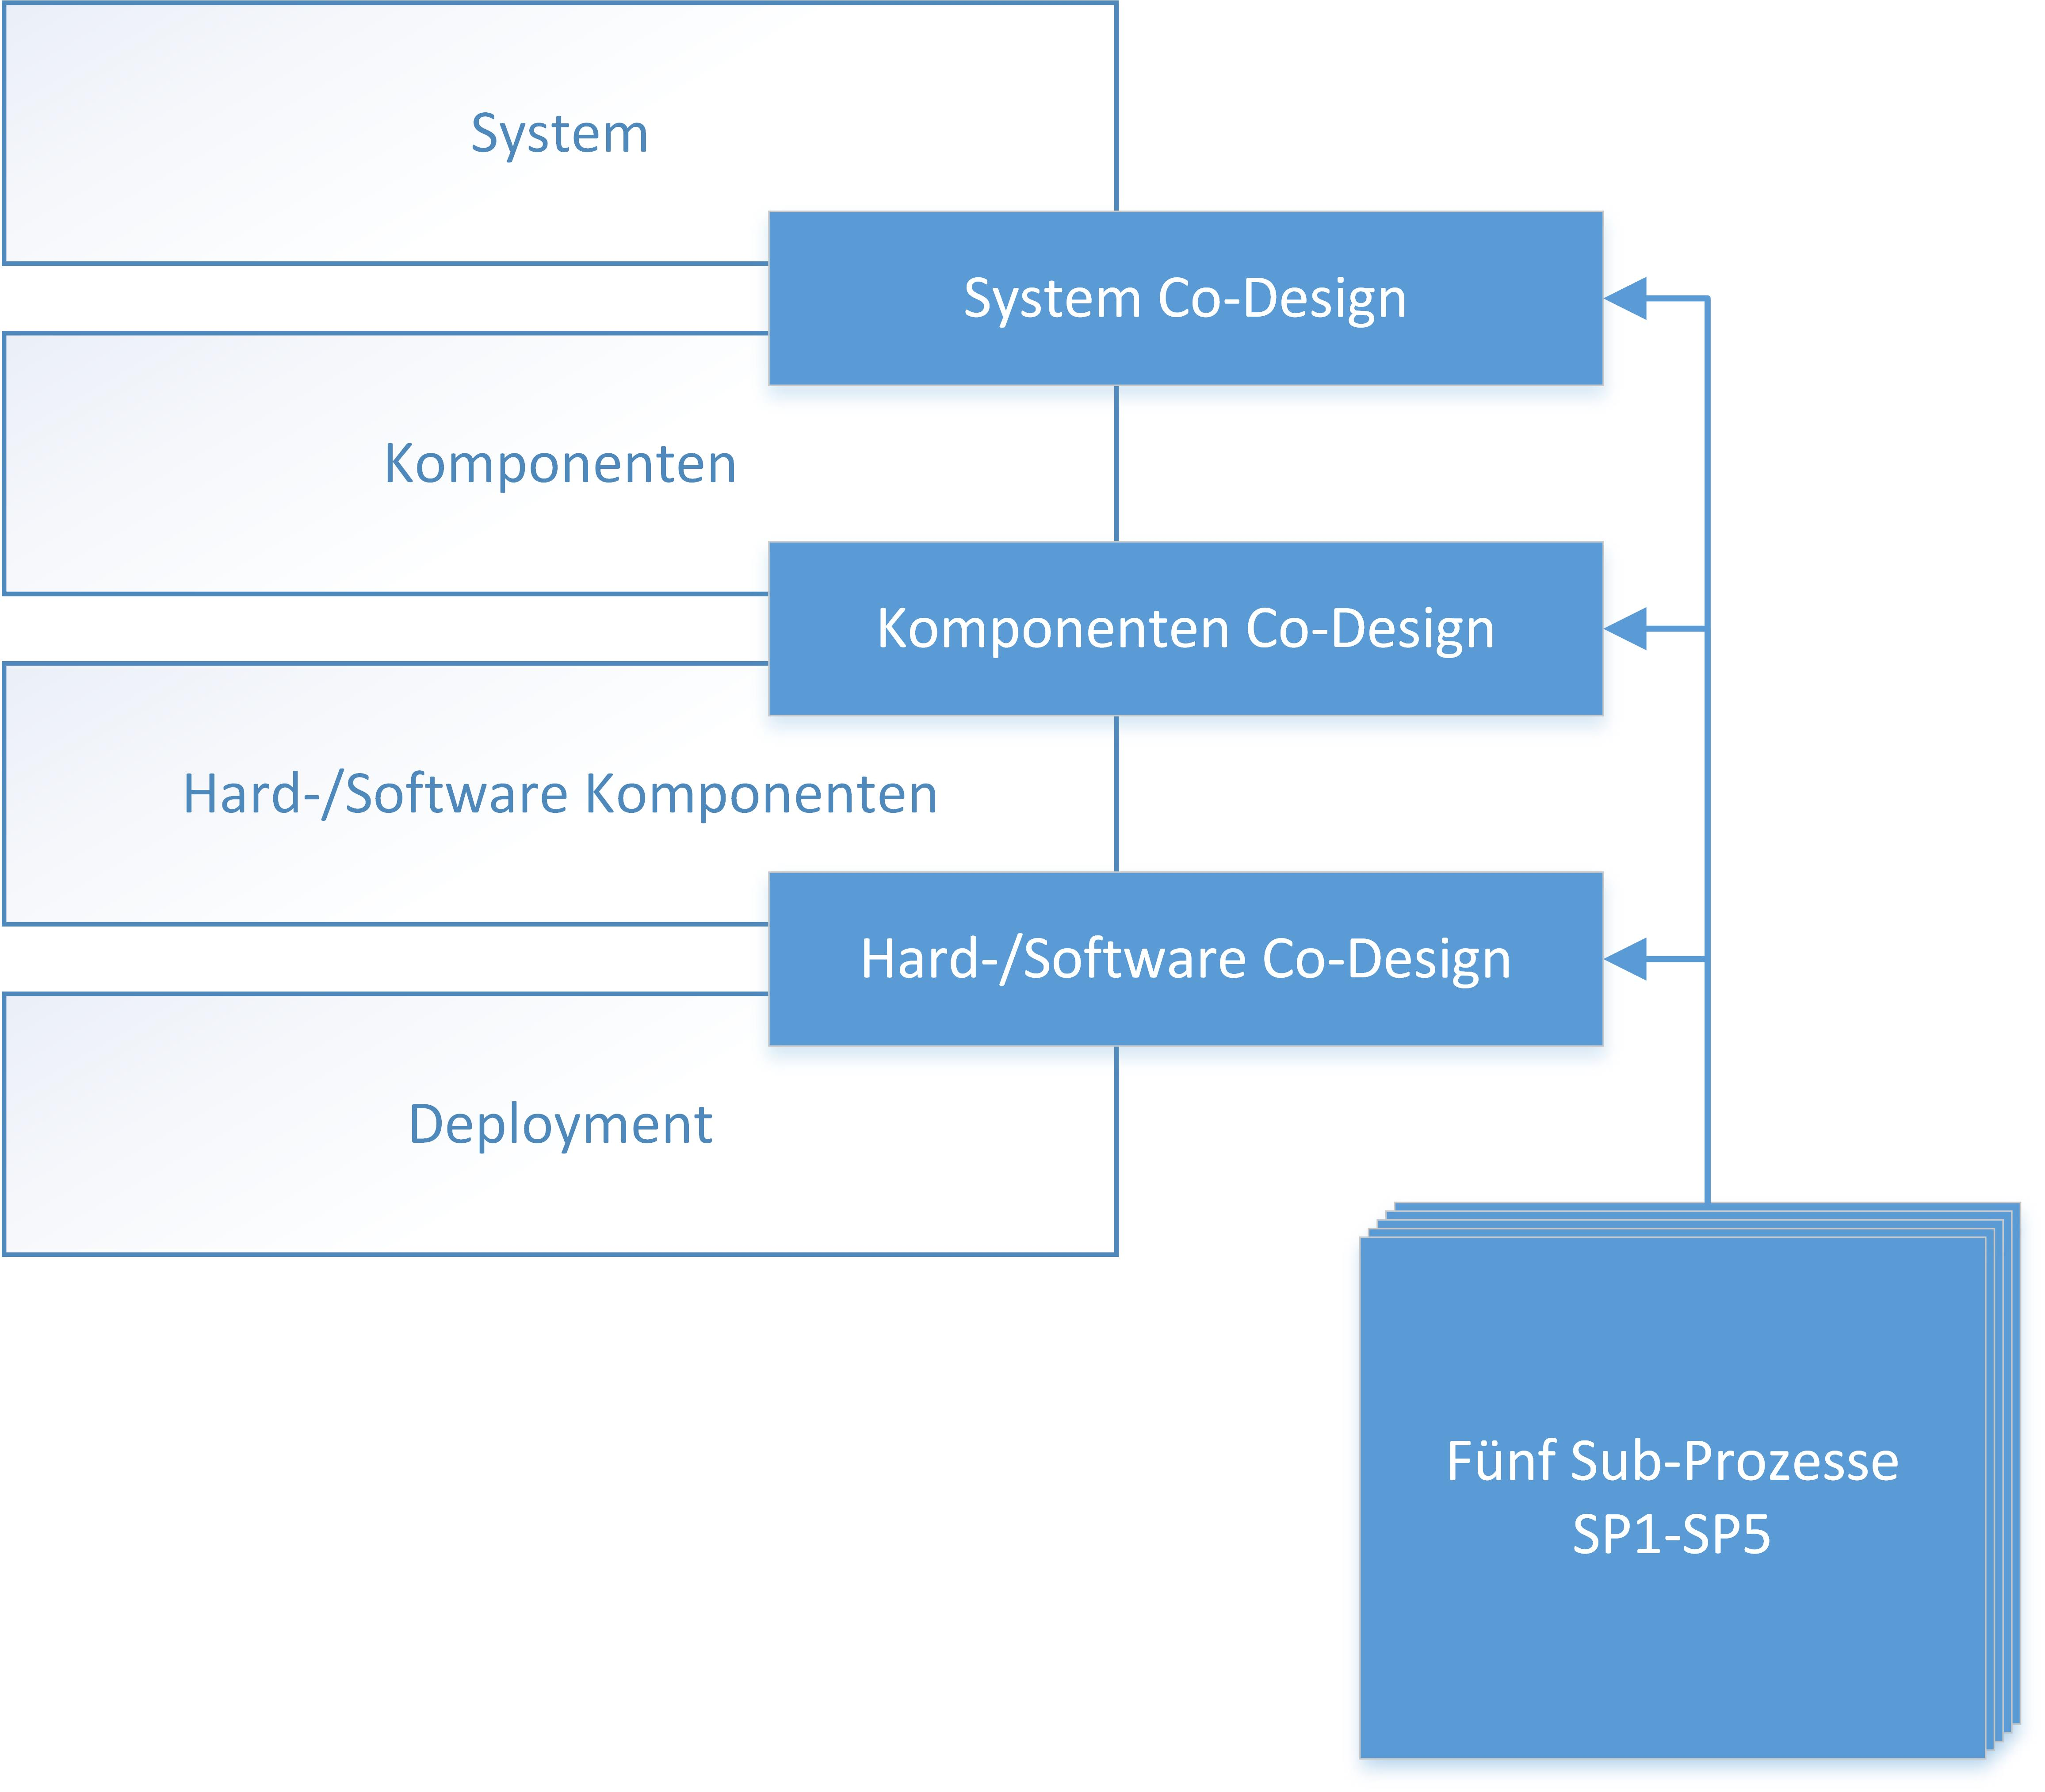
\includegraphics[scale=0.75]{COSMODREoverview.jpg} 
	\caption{Die fünf Subprozesse der COSMOD-RE Methode}\label{cosmodreow}
\end{figure}

In der Abbildung \ref{cosmodreow} ist schematisch dargestellt wie COSMOD-RE auszuführen ist. Es gibt vier Hierarchieebenen auf denen drei Co-Design Prozesse arbeiten die wiederum aus fünf Subprozessen bestehen.\\

\paragraph{Randbedingungen}
Bei der Anwendung von COSMOD-RE ist zu beachten, dass einige Bedingungen erfüllt sein müssen um die Methodik richtig anzuwenden:\\

\begin{itemize}
\item \emph{Definition einer Abstraktionshierarchie.} \\
Es gibt keine Richtlinien bezüglich der Definition der Abstraktionshierarchie. Dies bedeutet, dass die verwendeten Hierarchiestufen im jedem Projekt neu festgelegt werden müssen. Ferner ist hierbei von Relevanz, zu definieren, wo die Trennlinien zwischen verschiedenen Abstraktionsstufen sind \cite{sikora}.
\item \emph{Verknüpfung von Anforderungs- und Architekturmodellen.} \\
Da im Rahmen von COSMOD-RE Anforderungsartefakte und Architekturartefakte parallel entwickelt werden ist es notwendig diese miteinander zu verknüpfen um sie in den Kontext des Ziels der Software zu bringen. Für diese Verknüpfung ist die Anwendung von Methodenfragmenten notwendig \cite{sikora}.
\item \emph{Definition von Konsistenzbedingungen.} \\
Für die Definition von Konsistenzbedingungen gibt es keinen allgemeingültigen Ansatz. Daher ist es notwendig in jedem Projekt neu zu definieren, ob Konsistenz gegeben ist oder nicht \cite{sikora}.\\
\item \emph{Definition der System-Vision.} \\
Es muss eine System-Vision vorhanden sein um COSMOD-RE einsetzen zu können, da die Methode diese zu Anforderungen verfeinert \cite{Poh01}.\\
\end{itemize}

Sind diese Randbedingungen geklärt ist es möglich COSMOD-RE anzuwenden.\\

\paragraph{Eingabe}
Als Eingabe benötigt COSMOD-RE eine System-Vision. Dies bedeutet in initialen Gesprächen mit Stakeholdern muss bereits festgehalten sein, welche Vision von dem zu konzipierenden System gegeben ist. Die System-Vision ist vor allem in der Systemebene von Relevanz. auf den niedrigeren Ebenen sind die Ausgaben der oberen Ebenen bedeutsam.\\

\paragraph{Vorgehensmodell}
Um das Vorgehensmodell zu beschreiben muss zunächst geklärt werden, was unter den vier Hierarchieebenen zu verstehen ist. Danach werden die drei Co-Design Prozesse erläutert. Darauf folgt dann die Erläuterung der fünf Sub-Prozesse.\\

Die vier in Abbildung \ref{cosmodreow} dargestellten Hierarchieebenen sind:\\

\begin{itemize}
\item[1] System: Die Systemebene beschreibt die oberste Ebene, bei der in der Anforderungssicht das System als ganzes betrachtet wird. Im Fokus stehen dabei die Interaktionen mit dem System. Weiter werden funktionale Anforderungen und Qualitätsanforderungen erstellt, die sich auf das Gesamtsystem beziehen. Die Architektursicht konzentriert sich hier auf die Definition von externen Systemschnittstellen. Hier definierte Artefakte sollen primär die Kommunikation mit Stakeholdern unterstützen.
\item[2] Komponenten: Die Komponentenebene bezeichnet die Aufteilung des Systems in einzelne Komponenten aus denen sich dieses zusammensetzen soll. Für jede Komponente werden funktionale Anforderungen und Qualitätsanforderungen formuliert. Da in dieser Ebene die Basis für die Systemarchtitektur gelegt wird, hat die Kommunikation zwischen dem Software-Architekten und dem Requirements Engineer von besonderer Bedeutung. 
\item[3] Hard-/Software Komponenten: Auf dieser Ebene werden die zuvor erstellten Komponenten in Hard- und Software Komponenten aufgeteilt und weiter verfeinert. Anforderungen auf dieser Ebene sind somit speziell auf die Komponentenart bezogen. 
\item[4] Deployment: Auf dieser Ebene werden Softwarekomponenten programmierbaren Hardwarekomponeten zugeordnet. Anforderungen auf dieser Ebene beziehen sich auf das Deployment der Softwarekomponenten und ihrem Einfluss auf vorher definierte Anforderungen. 
\end{itemize}
Da die Zusammenarbeit zwischen Software-Architekt und Requirements Engineer vor allem in den obersten beiden Ebenen von Relevanz ist, sind die unteren beiden Ebenen in diesem Kontext zu vernachlässigen.\\

Ein Vorteil von COSMOD-RE ist unter anderem, dass Beziehung die sich über mehrere Hierarchieebenen erstrecken, nicht vernachlässigt werden. Dies ist durch die CO-Design Prozess möglich. Diese geben an, dass bei der Ausführung der Subprozesse mehrere Hierarchieebenen zu berücksichtigen sind. So wird beim System-Co-Design sowohl die Systemebene als auch die Komponentenebene betrachtet. Bei dem Komponenten Co-Design wird die Komponentenebene und diie Hard-/Software Komponentenebene betrachtet. Im Hard-/Software Co-Design wird die Hard-/Software Komponentenebene und die Deployment ebene berücksichtigt \cite{Poh02}. Jeder dieser drei CO-Design Prozesse führt dann die fünf Subprozesse aus.\\ 

Das grundsätzliche Vorgehen von COSMOD-RE ist, dass eine Systemvision unter der Verwendung von Szenarien und Zielen zu einer Menge von Systemartefakten verfeinert wird \cite{Poh01}. Hierfür nutzt die Methode fünf Subprozesse. \\

In Abbildung \ref{pro5} nach \cite{Poh01} sind diese zu sehen. 

\begin{figure}[h]
	\centering
	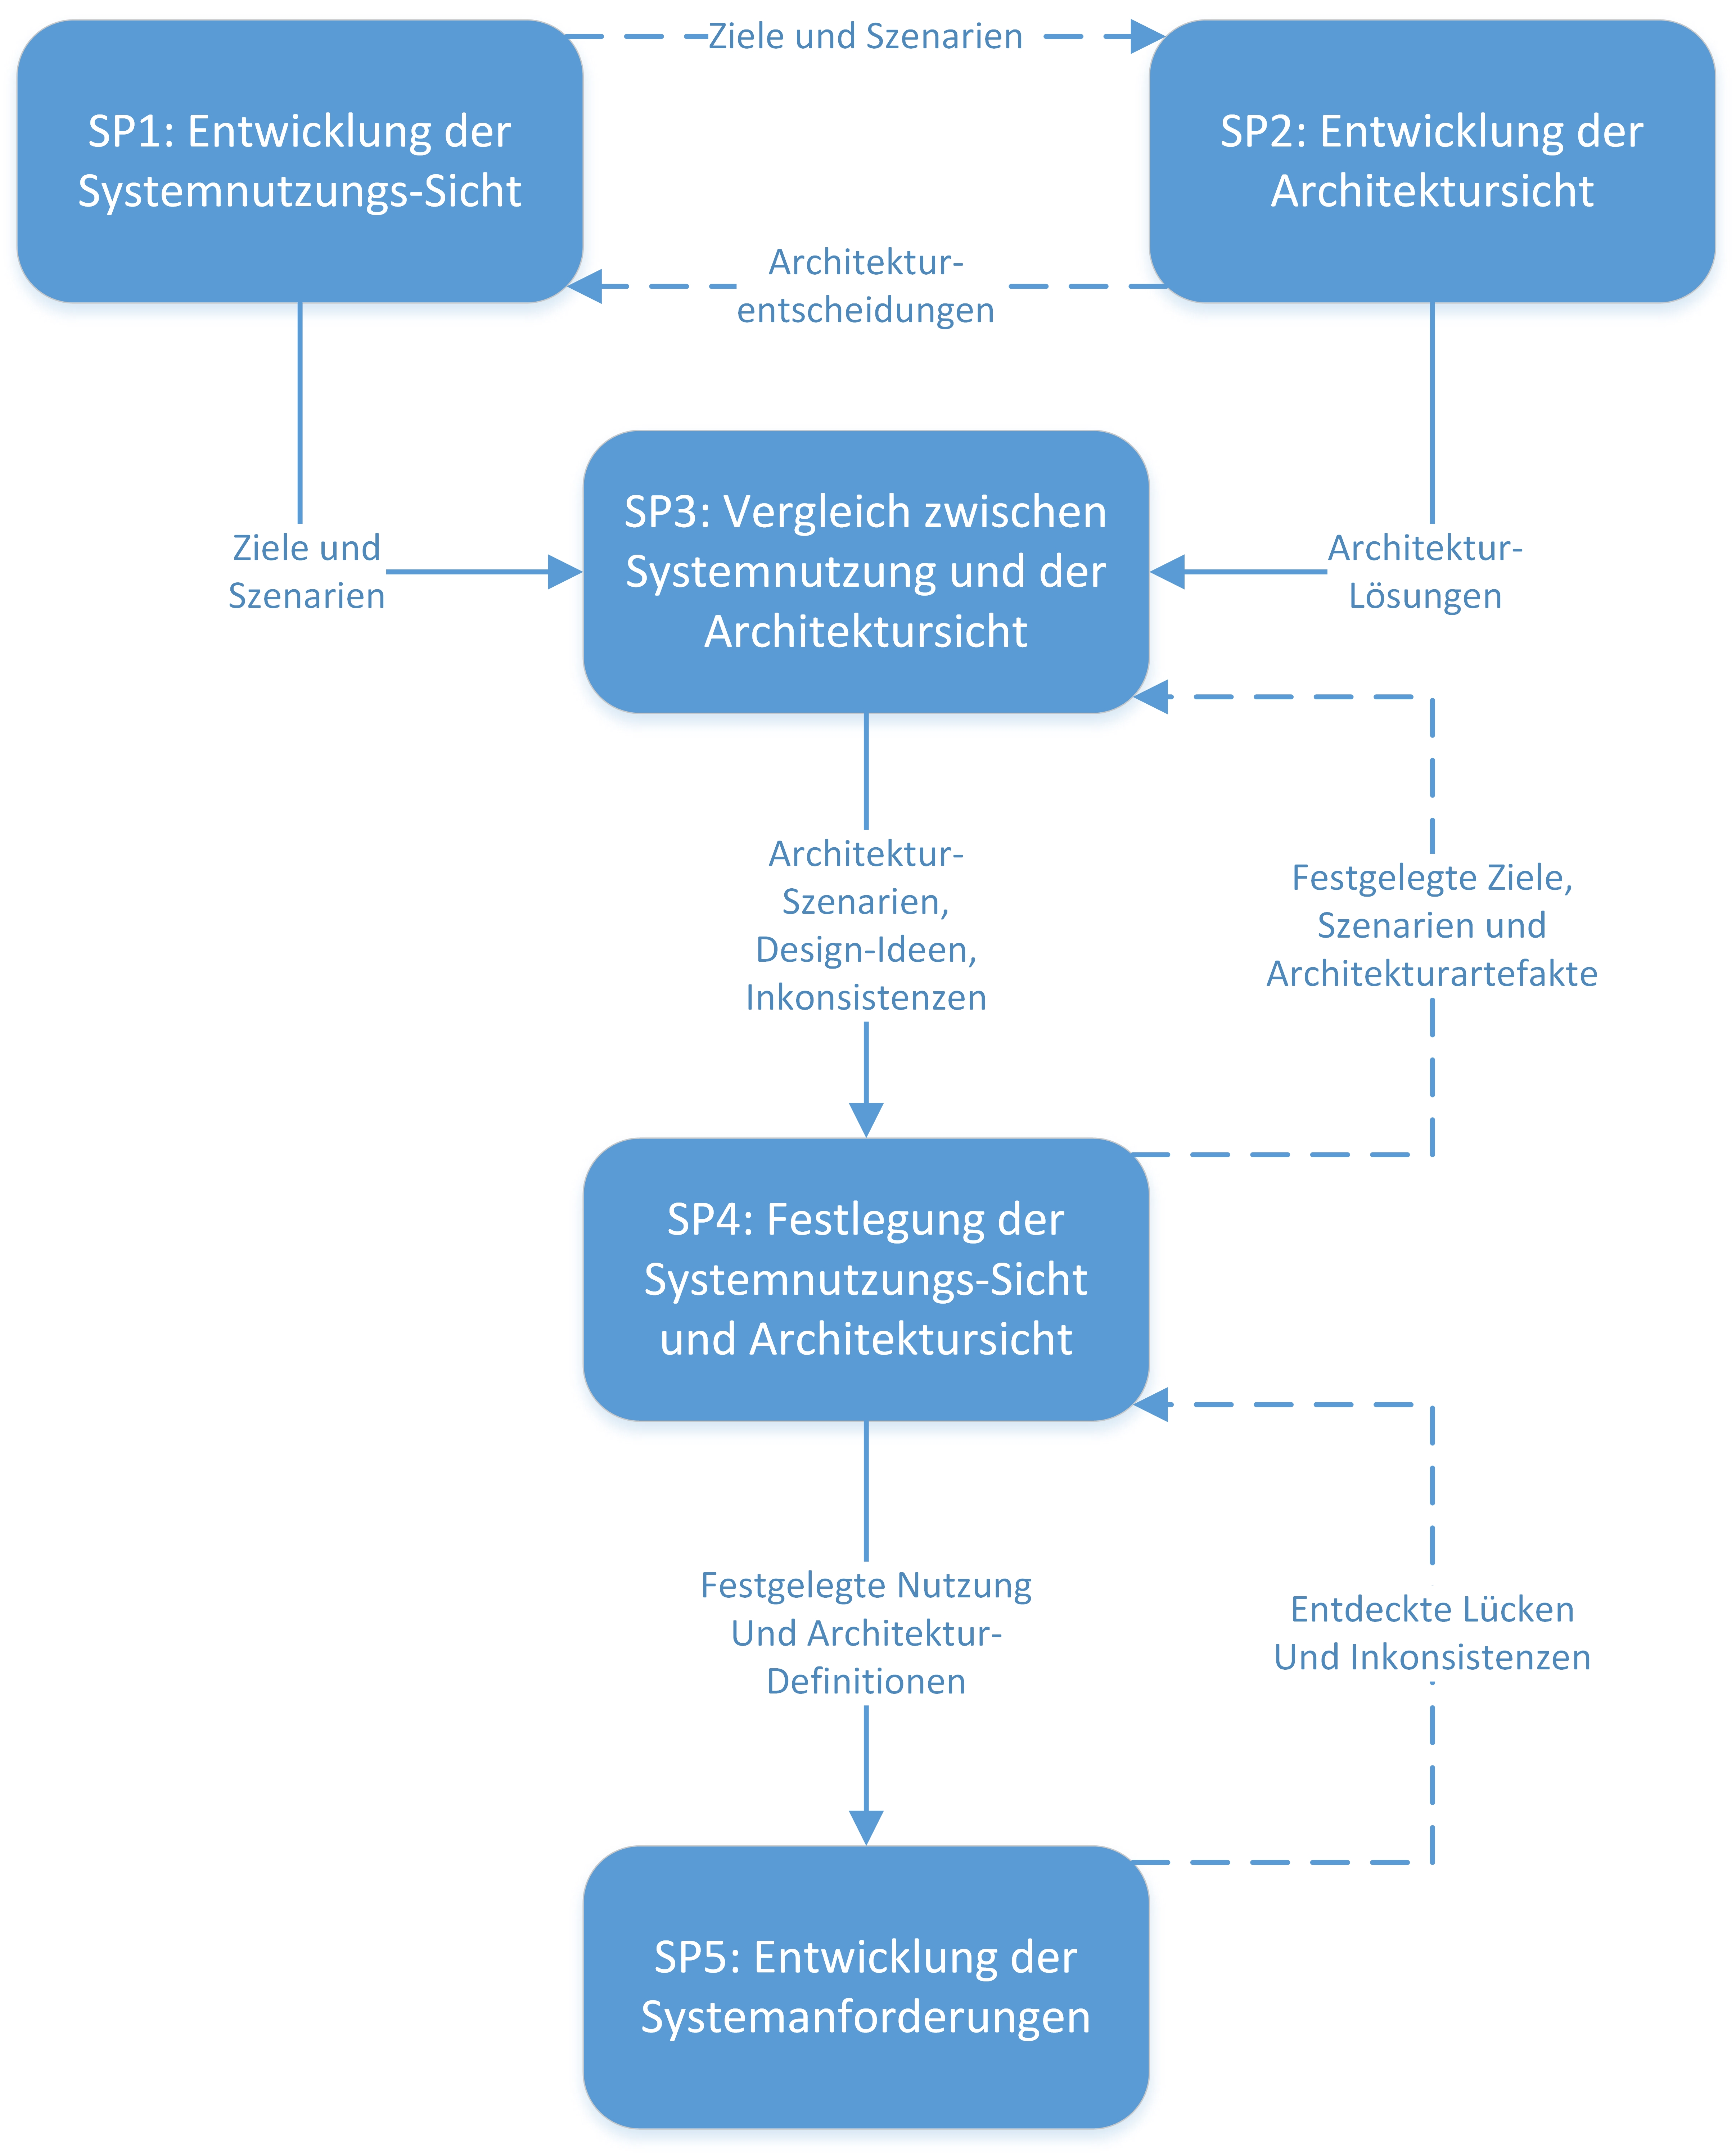
\includegraphics[scale=0.65]{COSMODRE5prozesse.jpg} 
	\caption{Die fünf Subprozesse der COSMOD-RE Methode}\label{pro5}
\end{figure}

\paragraph{SP1: Entwicklung der Systemnutzungs-Sicht}
Ziel dieses Subprozesses ist die Verfeinerung der System Vision. Zunächst sollen hier potentielle Akteure identifiziert werden. Daraufhin wird die System Vision in nutzerbezogene Unterziele aufgeteilt. Danach soll für jedes Ziel ein Nutzungs-Szenario gebildet werden, welches die Bedingungen für die Zielerreichung dokumentiert. In diesem Schritt ist als Eingabe die Eingabe der Methode, die System Vision, gegeben \cite{Poh01}. In diesem Prozess sind vor allem das Know-How des Requirements Engineer von Bedeutung. Dieser muss in Kooperation mit dem Kunden die Ziele dieses Subprozesses erreichen.\\

\paragraph{SP2: Entwicklung der Architektursicht}
Hauptziel dieses Subprozesses ist die Erzeugung grober Architekturlösungen für das geplante System. Eingabe in diesem Subprozess ist einerseits wieder die System Vision, andererseits jedoch die in SP1 gebildeten Systemnutzungs-Ziele und -Szenarien. Ausgabe dieses Prozesses ist ein grober Entwurf der Systemarchitektur \cite{Poh01}.\\

In diesem Subprozess werden vier Kernaktivitäten ausgeführt:\\

\begin{itemize}
\item \textit{Analyse der Systemziele und Nutzungs-Szenarien:} Ziel dieser Aktivität ist die Identifikation architekturrelevanter Aussagen in den Systemnutzungs-Zielen und Systemnutzungs-Szenarien. Diese können zum Beispiel hinweise auf spezielle Komponenten sein. 
\item \emph{Kreative Entwicklung neuer Architekturlösungen:} Ziel dieser Aktivität ist es innovative Lösungen für das System zu erarbeiten. Auch wenn die in SP1 erzeugten Ausgaben von Bedeutung sind, ist hier vor allem das Know-How der Software-Architekten von Relevanz. Das technisches Hintergrundwissen und der Einfallsreichtum sind von zentraler Bedeutung.
\item \emph{Bewertung der entwickelten Architekturlösungen:} Ziel dieser Aktivität ist die Auswertung der entwickelten Lösungsansätze um so die besten auszuwählen. 
\item \emph{Definition einer vorläufigen groben Architektur:} Ziel dieser Aktivität ist die Erzeugung einer (partiellen) Lösung basierend auf der zuvor ausgeführten Bewertung \cite{Poh01}.\\
\end{itemize} 

\paragraph{SP3: Vergleich zwischen Systemnutzungs-Sicht und Architektursicht}
Hauptziel dieses Subprozesses ist einerseits die Überprüfung, ob die Architektur die identifizierten Systemnutzungs-Ziele und Szenarien unterstützt und andererseits die Identifikation neuer Verwendungszwecke basierend auf der aktuellen groben System-Architektur \cite{Poh01}.\\

Die Überprüfung lässt sich auch betrachten als Vergleich der Ergebnisse von SP1 und SP2. Um die Systemnutzungs-Szenarien mit der Architektur zu vergleichen ist es notwendig die Systemnutzungs-Szenarien zu Architektur-Szenarien zu verfeinern. Diese Verfeinerung, die auch mithilfe von Message-Sequence-Charts durchgeführt werden kann, wird üblicherweise über drei Schritte durchgeführt \cite{Poh01}.\\

\begin{itemize}
\item Das System wird in eine Untermenge funktionaler Anforderungen verfeinert, welche in der groben Architektur definiert werden.
\item Jeder Systemnutzung wird eine funktionale Komponente zugeordnet, die verantwortlich für die Realisierung der Interaktion mit externen Akteuren ist. 
\item System interne Interaktionen, die externe Interaktionen ermöglichen, werden definiert \cite{Poh01}.\\
\end{itemize}

\paragraph{SP4: Festlegung der Systemnutzungs-Sicht und Architektursicht}
Wie auch in SP3 gibt es hier zwei zentrale Ziele. Einerseits sollen die in SP1 erzeugten Systemnutzungs-Ziele und -Szenarien mithilfe der Erkenntnisse aus SP3 verbessert und angepasst werden und andererseits soll die in SP2 gebildete grobe Architektur mithilfe der Erkenntnisse aus SP3 verbessert und angepasst werden \cite{Poh01}.\\

Hierfür muss zunächst bei den Ausgaben von SP3 überprüft werden, ob sie zur Verbesserung der Ergebnisse von SP1 und SP2 geeignet sind. Hierfür ist es angemessen ein System zur Kategorisierung einzuführen, über das entschieden werden kann ob eine Verbesserung notwendig oder nicht notwendig ist. Danach werden die Ergebnisse von SP3 priorisiert. Hier wird überprüft welche Verbesserung zuerst umgesetzt werden sollte und welche nicht direkt notwendig sind. Zuletzt werden die Verbesserungen umgesetzt. Hier ist jedoch zu beachten, dass Verbesserungen neue Ideen hervorrufen könnten oder Inkonsistenzen erzeugen könnten. Daher kann es notwendig sein SP3 zu wiederholen. Diese Iteration ist solange durchzuführen, bis die Ergebnisse angemessen angeordnet und stabil sind \cite{Poh01}.\\

\paragraph{SP5: Entwicklung der Systemanforderungen}
Hauptziel dieses Subprozesses ist die Spezifikation detaillierter Systemanforderungen. Grundlage für die Spezifikation sind die Systemnutzungs-Sicht und die Architektursicht. Mithilfe von Zielen, Szenarien und dem groben Architekturentwurf ist es möglich detaillierte Anforderungen zu formulieren und in der Spezifikation aufzuführen.\\

\paragraph{Ausgabe}
Ausgabe der Methode ist eine kompakte Menge von System-Nutzung-Zielen, System-Interaktions-Szenarien und grobe Architekturartefakte. Ferner wird eine detaillierte System-Anforderungsspezifikation generiert.\\

Vor allem im Rahmen der fünf Subprozesse werden folgende Artefakte generiert:\\

\begin{figure}[h]
	\centering
	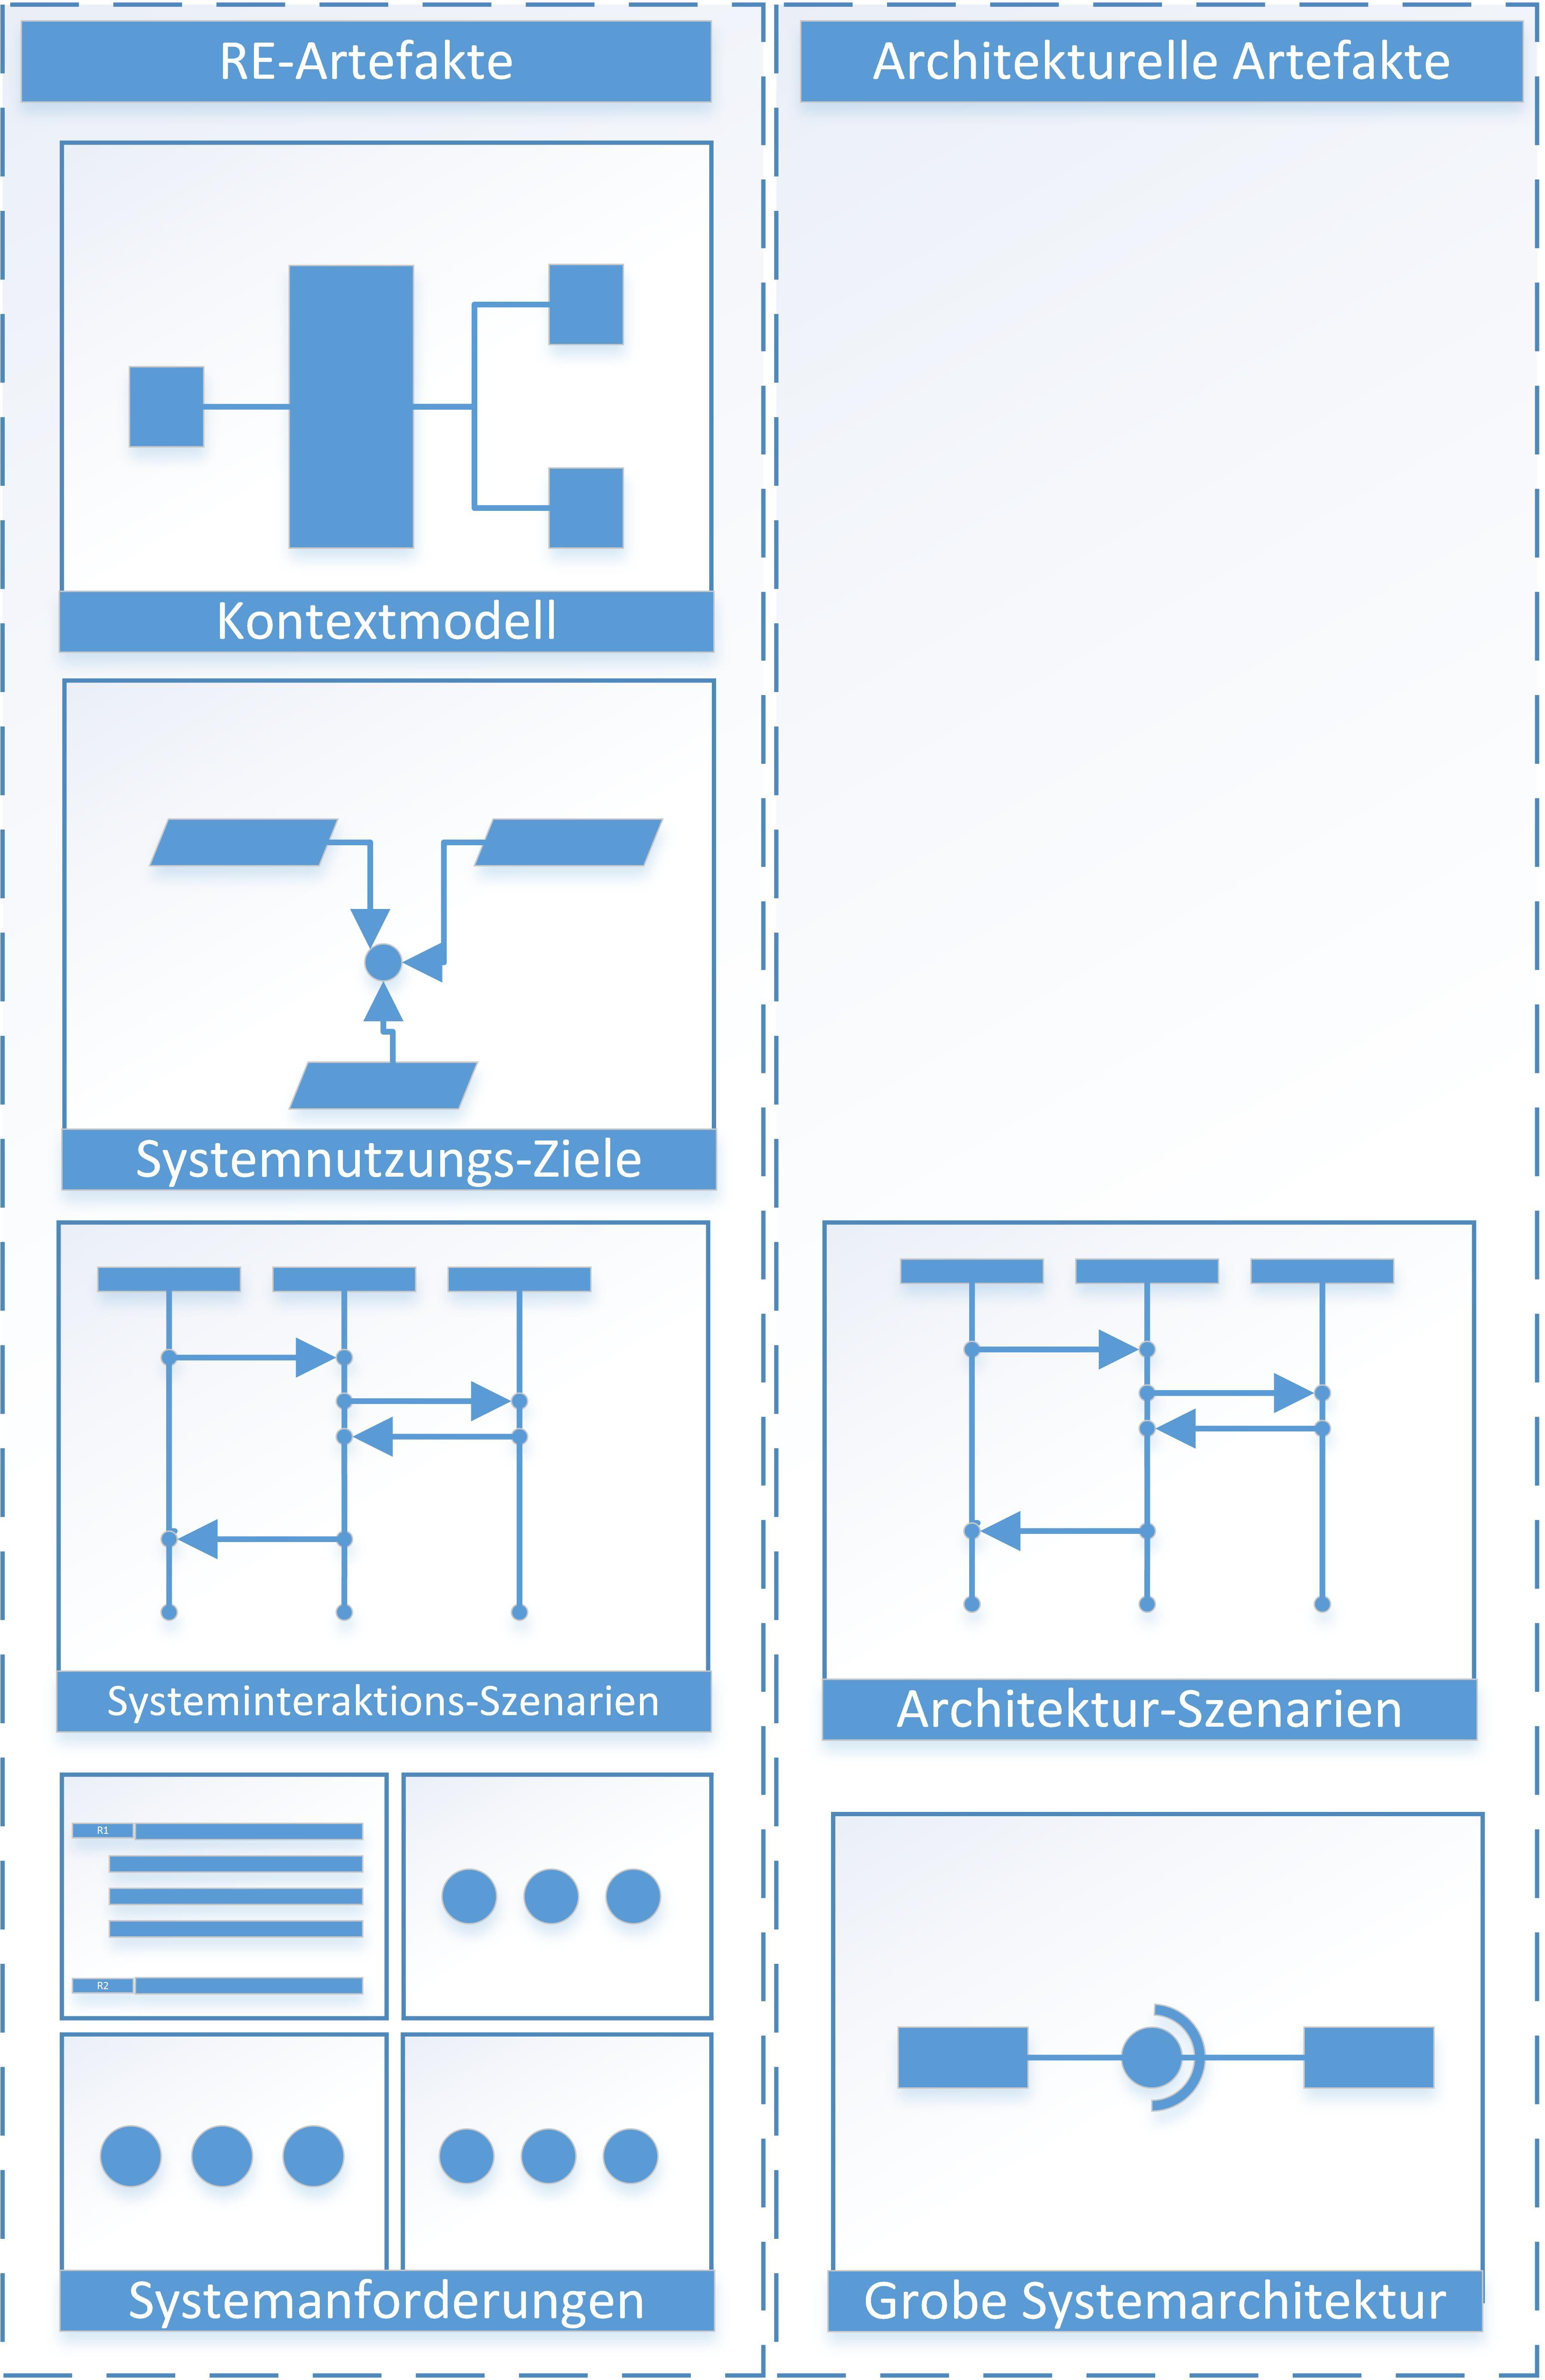
\includegraphics[scale=0.8]{artefakte.jpg} 
	\caption{Die Artefakte der COSMOD-RE Methode}\label{art}
\end{figure}

\begin{itemize}
\item Kontextmodell:\\
Das Kontextmodell dokumentiert die beabsichtigte Einbettung des Systems in seine Systemumgebung. Es werden externe Akteure definiert, die mit dem System interagieren. Ein Akteur kann hierbei ein Mensch oder ein System sein. Ferner wird modelliert, wie Akteure mit dem System interagieren \cite{Poh01}.
\item Systemnutzungs-Ziele:\\
Systemnutzungs-Ziele verfeiner die Systemvision. Ein Systemnutzungs-Ziel dokumentiert eine Eigenschaft des Systems in Bezug zu externen Akteuren, die das System nutzen. Ein Ziel kann hierbei in Unterziele unterteilt werden wodurch eine Hierarchie von Zielen möglich ist \cite{Poh01}.  
\item Systeminteraktions-Szenarien:\\
Mit diesen Szenarien werden Interaktionen von Akteuuren mit dem System dokumentiert. Für die Dokumentation solcher Szenarien bieten sich modellbasierte Ansätze an \cite{Poh01}.
\item Architektur-Szenarien:\\
Mithilfe dieser Szenarien werden Interaktionen innerhalb des Systems dokumentiert. Hiermit sind vor allem Interaktionen zwischen Systemkomponenten gemeint \cite{Poh01}. 
\item Grobe System-Architektur:\\
Hier wird eine Zerlegung der System-Architektur in eine Menge funktionaler Komponenten vollzogen, die über Schnittstellen verknüpft sind \cite{Poh01}.
\item Systemanforderungen:
Als Systemanforderungen werden hier funktionale, strukturelle oder verhaltensbezogene Anforderungen gemeint. Weiter werden Qualitätsanforderungen die sich beispielsweise auf Performance oder Sicherheit beziehen spezifiziert \cite{Poh01}.\\
\end{itemize}

Durch die iterative Verbesserung der Anforderungen und Systemarchitektur ist es abhängig von der Anzahl der Iterationen möglich ein Abbild der System-Vision zu erzeugen, sofern diese zu Beginn korrekt definiert wurde.